\documentclass[11pt]{ctexart}

% 插入宏包
\usepackage{graphicx} % Required for inserting images
\usepackage{geometry} % 设置页边距
\usepackage{lipsum} % 生成虚拟文本
\usepackage{fancyhdr} 
\setlength{\headheight}{14pt}% 自定义页眉和页脚
\usepackage{booktabs} % 插入三线表
\usepackage{lastpage} % 解决总页数显示问题
\usepackage{amsmath,amsfonts,amsthm} % 常用数学公式指令、数学公式、提供证明环境
\usepackage{bm} % 数学字体加粗
\usepackage{mathrsfs} % 提供特殊的数学花体
\usepackage{amssymb, ,hyperref, framed, color, enumerate}
\usepackage{bbding} % 打叉、打勾

% Custom counter for problems
\newcounter{problemname}

% Environment for problems
\definecolor{shadecolor}{RGB}{241, 241, 255}

\newenvironment{problem}{\begin{shaded}\stepcounter{problemname}\par\noindent\textbf{习题}\arabic{problemname}.}{\end{shaded}\par}


% Environment for solutions
\newenvironment{solution}{\par\noindent\textbf{解答. }}{\par}

% Environment for notes
\newenvironment{note}{\par\noindent\textbf{习题\arabic{problemname}的注记. }}{\par}

% Reset problem counter at each subsection
\usepackage{titlesec}
\titleformat{\subsection}{\normalfont\large\bfseries}{\thesubsection}{1em}{\setcounter{problemname}{0}}

% 设置文章格式
\geometry{left=2.5cm,right=2.5cm,top=3cm,bottom=3cm}
\pagestyle{fancy} % 使用fancyhdr宏包定义页眉页脚
\fancyhf{} % 清空默认的页眉和页脚设置
\linespread{1.5}
\chead{《固体物理学(胡安版)》作业}
\cfoot{第 \thepage 页(共 \pageref{LastPage}页)}

% 信息栏
\title{\Huge\textbf{固体物理学作业}}
\author{Charles Luo}
\date{\today}

% 正文区
\begin{document}
\maketitle
\newpage
\tableofcontents
\newpage

\section{第一章习题}

\begin{problem}
    在正交直角坐标系中,若矢量 $\mathbf{R}_n = n_1\,\mathbf{i} + n_2\,\mathbf{j} + n_3\,\mathbf{k}$, 其中 $\mathbf{i},\,\mathbf{j},\,\mathbf{k}$
    为单位矢量,$n_i\ (i = 1,2,3)$ 为整数。问下列情况属于什么点阵?
    \begin{enumerate}[(a)]
        \item 当 $n_i$ 为全奇加全偶时;
        \item 当 $n_i$ 之和为偶数时。
    \end{enumerate}
\end{problem}
\begin{solution}
    \begin{enumerate}[(a)]
        \item 据题意,全奇加全偶应是两个布拉维格子的叠加。 \\
              若 $n_i\ (i = 1,2,3)$ 全为偶数,可以提取公因子 $2$ 得到 $\mathbf{R}_n = n_1^\prime\left(2\mathbf{i}\right) + n_2^\prime\left(2\mathbf{j}\right) + n_3^\prime\left(2\mathbf{k}\right)$,
              此时 $n_i^\prime\ (i = 1,2,3)$ 为整数,对应简单立方点阵,格矢长度为 $2$ 个单位长度。 \\
              同理可得 $n_i\ (i = 1,2,3)$ 全为奇数时也为简单立方点阵,可由全为偶数时点阵沿 $\left(1,1,1\right)$ 方向平移移一个单位长度得到。 \\
              二者的嵌套为体心立方点阵。
        \item 据题意,$n_1 + n_2 + n_3 = 2k,\ k\in\mathbb{N}$。 \\
              不妨取 $k = 1$ 和 $k = 2$ 来猜测,可以得到格点坐标为 $\left(1,1,0\right),\cdots,\left(0,1,1\right),\left(2,0,0\right),\cdots,\left(0,0,2\right)$.
              为面心立方点阵。
    \end{enumerate}
\end{solution}
\begin{note}
    \begin{itemize}
        \item (b)可取 $k_1 = k - n_1, k_2 = k - n_2, k_3 = k - n_1 - n_2$, 
                 得到 $\mathbf{R}_n = \left(k_2 + k_3\right)\mathbf{i} + \left(k_3 + k_1\right)\mathbf{j} + \left(k_1 + k_2\right)\mathbf{k}$.
    \end{itemize}
\end{note}

\begin{problem}
    分别证明:
    \begin{enumerate}[(a)]
        \item 面心立方(fcc)和体心立方(bcc)点阵的惯用初基元胞三基矢间夹角 $\theta$ 相等,
              对fcc为 $60^\circ$ ,对bcc为 $109^\circ27^\prime$;
        \item 在金刚石结构中,作任一原子与其四个最近邻原子的连线。证明任意两条线之间夹角 $\theta$ 均为 \\[12pt]
              $\arccos{\left(-\dfrac{1}{3}\right)} = 109^\circ27^\prime$。
    \end{enumerate}
\end{problem}
\begin{solution}
    \begin{enumerate}[(a)]
        \item fcc 三个基矢为 $\mathbf{a_1} = \left(0,\dfrac{1}{2},\dfrac{1}{2}\right),\mathbf{a_2} = \left(\dfrac{1}{2},0,\dfrac{1}{2}\right),\mathbf{a_3} = \left(\dfrac{1}{2},\dfrac{1}{2},0\right)$. \\[12pt]
              故 $\cos{\theta} = \dfrac{\mathbf{a_1}\cdot\mathbf{a_2}}{\left|\mathbf{a_1}\right|\left|\mathbf{a_2}\right|} = \dfrac{\mathbf{a_2}\cdot\mathbf{a_3}}{\left|\mathbf{a_2}\right|\left|\mathbf{a_3}\right|} = \dfrac{\mathbf{a_3}\cdot\mathbf{a_1}}{\left|\mathbf{a_3}\right|\left|\mathbf{a_1}\right|} = \dfrac{1}{2}$,即 $\theta = 60^\circ$. \\[12pt]
              bcc 三个基矢为 $\mathbf{a_1} = \left(-\dfrac{1}{2},\dfrac{1}{2},\dfrac{1}{2}\right),\mathbf{a_2} = \left(\dfrac{1}{2},-\dfrac{1}{2},\dfrac{1}{2}\right),\mathbf{a_3} = \left(\dfrac{1}{2},\dfrac{1}{2},-\dfrac{1}{2}\right)$. \\[12pt]
              故 $\cos{\theta} = \dfrac{\mathbf{a_1}\cdot\mathbf{a_2}}{\left|\mathbf{a_1}\right|\left|\mathbf{a_2}\right|} = \dfrac{\mathbf{a_2}\cdot\mathbf{a_3}}{\left|\mathbf{a_2}\right|\left|\mathbf{a_3}\right|} = \dfrac{\mathbf{a_3}\cdot\mathbf{a_1}}{\left|\mathbf{a_3}\right|\left|\mathbf{a_1}\right|} = -\dfrac{1}{3}$,即 $\theta = \arccos{\left(-\dfrac{1}{3}\right)} = 109^\circ27^\prime$.
        \item 金刚石结构中坐标为 $\left(\dfrac{1}{4},\dfrac{1}{4},\dfrac{1}{4}\right)$ 的原子相邻的4个原子坐标分别为 $\left(0,0,0\right),\left(0,\dfrac{1}{2},\dfrac{1}{2}\right),\left(\dfrac{1}{2},0,\dfrac{1}{2}\right),$ \\[12pt] 
              $\left(\dfrac{1}{2},\dfrac{1}{2},0\right)$. 邻边 $\mathbf{l_1} = \left(-\dfrac{1}{4},-\dfrac{1}{4},-\dfrac{1}{4}\right),\mathbf{l_2} = \left(-\dfrac{1}{4},\dfrac{1}{4},\dfrac{1}{4}\right),\mathbf{l_3} = \left(\dfrac{1}{4},-\dfrac{1}{4},\dfrac{1}{4}\right),\mathbf{l_4} = \left(\dfrac{1}{4},\dfrac{1}{4},-\dfrac{1}{4}\right)$. \\[12pt]
              故 $\cos{\theta} = \dfrac{\mathbf{l_1}\cdot\mathbf{l_2}}{\left|\mathbf{l_1}\right|\left|\mathbf{l_2}\right|} = \dfrac{\mathbf{l_2}\cdot\mathbf{l_3}}{\left|\mathbf{l_2}\right|\left|\mathbf{l_3}\right|} = \dfrac{\mathbf{l_3}\cdot\mathbf{l_4}}{\left|\mathbf{l_3}\right|\left|\mathbf{l_4}\right|} = \dfrac{\mathbf{l_4}\cdot\mathbf{l_1}}{\left|\mathbf{l_4}\right|\left|\mathbf{l_1}\right|} = -\dfrac{1}{3}$,即 $\theta = \arccos{\left(-\dfrac{1}{3}\right)} = 109^\circ27^\prime$.
    \end{enumerate}
\end{solution}

\begin{problem}
    证明在六角晶系中米勒指数为 $(hkl)$ 的晶面族间距为
    $$d = \left[\frac{4}{3}\left(\frac{h^2 + hk + k^2}{a^2} + \frac{l^2}{c^2}\right)\right]^{-\frac{1}{2}}.$$
\end{problem}
\begin{solution}
    米勒指数以单胞的三条棱为坐标系. \\[12pt]
    正点阵的一族晶面 $\left(hkl\right)$ 垂直于倒格矢 $\mathbf{K_h} = h\mathbf{b_1} + k\mathbf{b_2} + l\mathbf{b_3}$,晶面间距 $\dfrac{2\pi}{\left|\mathbf{K_h}\right|}$. \\[12pt]
    在六角晶系中 $\mathbf{a} = \left(a,0,0\right),\mathbf{b} = \left(-\dfrac{1}{2}a,\dfrac{\sqrt{3}}{2}a,0\right),\mathbf{c} = \left(0,0,c\right)$. \\[12pt]
    求倒点阵基矢:\\[12pt]
    $\mathbf{b_1} = 2\pi\dfrac{\mathbf{a_2}\times\mathbf{a_3}}{\mathbf{a_1}\cdot\left(\mathbf{a_2}\times\mathbf{a_3}\right)} = \dfrac{2\pi}{a}\left(1,\dfrac{\sqrt{3}}{3},0\right)$. \\[12pt]
    $\mathbf{b_2} = 2\pi\dfrac{\mathbf{a_3}\times\mathbf{a_1}}{\mathbf{a_1}\cdot\left(\mathbf{a_2}\times\mathbf{a_3}\right)} = \dfrac{2\pi}{a}\left(0,\dfrac{2\sqrt{3}}{3},0\right)$. \\[12pt]
    $\mathbf{b_3} = 2\pi\dfrac{\mathbf{a_1}\times\mathbf{a_2}}{\mathbf{a_1}\cdot\left(\mathbf{a_2}\times\mathbf{a_3}\right)} = \dfrac{2\pi}{c}\left(0,0,1\right)$. \\[12pt]
    倒格矢 $\mathbf{K_h} = \left(\dfrac{2\pi}{a}h,\dfrac{2\sqrt{3}\pi}{3a}h+\dfrac{4\sqrt{3}\pi}{3a}k,\dfrac{2\pi}{c}l\right)$, 故 $\displaystyle d = \dfrac{2\pi}{\left|\mathbf{K_h}\right|} = \left[\frac{4}{3}\left(\frac{h^2 + hk + k^2}{a^2} + \frac{l^2}{c^2}\right)\right]^{-\frac{1}{2}}.$
\end{solution}

\begin{problem}
    证明底心正交点阵的倒点阵仍为底心正交点阵。
\end{problem}
\begin{solution}
    底心正交阵基矢 $\mathbf{a_1} = \left(a,0,0\right),\mathbf{a_2} = \left(\dfrac{a}{2},\dfrac{b}{2},0\right),\mathbf{a_3} = \left(0,0,c\right)$. \\[12pt]
    倒点阵基矢: \\[12pt]
    $\mathbf{b_1} = 2\pi\dfrac{\mathbf{a_2}\times\mathbf{a_3}}{\mathbf{a_1}\cdot\left(\mathbf{a_2}\times\mathbf{a_3}\right)} = 2\pi\left(\dfrac{1}{a},-\dfrac{1}{b},0\right)$. \\[12pt]
    $\mathbf{b_2} = 2\pi\dfrac{\mathbf{a_3}\times\mathbf{a_1}}{\mathbf{a_1}\cdot\left(\mathbf{a_2}\times\mathbf{a_3}\right)} = 2\pi\left(0,\dfrac{2\pi}{b},0\right)$. \\[12pt]
    $\mathbf{b_3} = 2\pi\dfrac{\mathbf{a_1}\times\mathbf{a_2}}{\mathbf{a_1}\cdot\left(\mathbf{a_2}\times\mathbf{a_3}\right)} = 2\pi\left(0,0,\dfrac{1}{c}\right)$. \\[12pt]
    倒点阵仍为底心正交阵,底面边长为 $\dfrac{4\pi}{a}$ 和 $\dfrac{4\pi}{b}$,高为 $\dfrac{2\pi}{c}$.
\end{solution}

\begin{problem}
    试证明具有四面体对称性的晶体,其介电常量为一标量介电常量:
    $$\bm{\varepsilon}_{\alpha\beta} = \varepsilon_0\delta_{\alpha\beta}.$$
\end{problem}
\begin{solution}
    根据电动力学有
    $$
    \mathbf{D} = \bm{\varepsilon}\mathbf{E},\ \bm{\varepsilon} = 
    \begin{pmatrix}
        \varepsilon_{11} & \varepsilon_{12} & \varepsilon_{13} \\
        \varepsilon_{21} & \varepsilon_{22} & \varepsilon_{23} \\
        \varepsilon_{31} & \varepsilon_{32} & \varepsilon_{33} \\
    \end{pmatrix}.
    $$
    四面体对称性包括三个四重反演轴,绕 x,y,z 轴旋转的操作分别记为 $\mathbf{A}_x,\mathbf{A}_y,\mathbf{A}_z$,反演操作记为 $\mathbf{I}$.
    $$
    \mathbf{A}_x = 
    \begin{pmatrix}
        1 & 0 & 0 \\
        0 & 0 & 1 \\
        0 & -1 & 0 \\
    \end{pmatrix},
    \mathbf{A}_y = 
    \begin{pmatrix}
        0 & 0 & -1 \\
        0 & 1 & 1 \\
        1 & 0 & 0 \\
    \end{pmatrix},
    \mathbf{A}_z = 
    \begin{pmatrix}
        0 & -1 & 0 \\
        1 & 0 & 0 \\
        0 & 0 & 1 \\
    \end{pmatrix},
    \mathbf{I} = 
    \begin{pmatrix}
        -1 & 0 & 0 \\
        0 & -1 & 0 \\
        0 & 0 & -1 \\
    \end{pmatrix}.
    $$
    由题意,应有 $\left(\mathbf{I}\mathbf{A}_x\right)\bm{\varepsilon}\left(\mathbf{I}\mathbf{A}_x\right)^T = \bm{\varepsilon}$.即
    $$
    \begin{pmatrix}
        -1 & 0 & 0 \\
        0 & 0 & -1 \\
        0 & 1 & 0 \\
    \end{pmatrix}
    \begin{pmatrix}
        \varepsilon_{11} & \varepsilon_{12} & \varepsilon_{13} \\
        \varepsilon_{21} & \varepsilon_{22} & \varepsilon_{23} \\
        \varepsilon_{31} & \varepsilon_{32} & \varepsilon_{33} \\
    \end{pmatrix}
    \begin{pmatrix}
        -1 & 0 & 0 \\
        0 & 0 & 1 \\
        0 & -1 & 0 \\
    \end{pmatrix} = 
    \begin{pmatrix}
        \varepsilon_{11} & \varepsilon_{12} & \varepsilon_{13} \\
        \varepsilon_{21} & \varepsilon_{22} & \varepsilon_{23} \\
        \varepsilon_{31} & \varepsilon_{32} & \varepsilon_{33} \\
    \end{pmatrix}
    $$
    可得 $\varepsilon_{13} = \varepsilon_{12} = 0,\varepsilon_{21} = -\varepsilon_{31},\varepsilon_{32} = -\varepsilon_{23},\varepsilon_{22} = \varepsilon_{33}$. \\
    利用 $\left(\mathbf{I}\mathbf{A}_y\right)\bm{\varepsilon}\left(\mathbf{I}\mathbf{A}_y\right)^T = \bm{\varepsilon}$ 及  $\left(\mathbf{I}\mathbf{A}_z\right)\bm{\varepsilon}\left(\mathbf{I}\mathbf{A}_z\right)^T = \bm{\varepsilon}$ 可知 
    $\bm{\varepsilon}_{\alpha\beta} = \varepsilon_0\delta_{\alpha\beta}$.
\end{solution}

\begin{problem}
    若 $AB_3$ 的立方结构如图所示,设 $A$ 原子的散射因子为 $f_A(\mathbf{K}_{hkl})$,
    $B$ 原子的散射因子 $f_B(\mathbf{K}_{hkl})$.
    \begin{enumerate}[(a)]
        \item 求其几何结构因子 $F(\mathbf{K}_{hkl}) = ?$
        \item 找出 $\left(hkl\right)$ 衍射面的 X射线衍射强度分别在什么情况下有
              $$ 
              I\left(\mathbf{K}_{hkl}\right)\propto\begin{cases}
              \left|f_A(\mathbf{K}_{hkl}) + 3f_B(\mathbf{K}_{hkl})\right|^2 \\
              \left|f_A(\mathbf{K}_{hkl}) - f_B(\mathbf{K}_{hkl})\right|^2
              \end{cases}
              $$
        \item 设 $f_A(\mathbf{K}_{hkl}) = f_B(\mathbf{K}_{hkl})$,问衍射面指数中哪些反射消失?试举出五种最简单的。
    \end{enumerate}
\end{problem}
\begin{solution}
    \begin{enumerate}[(a)]
        \item 取原子坐标 A $\left(0,0,0\right)$ , B $\left(\dfrac{1}{2},\dfrac{1}{2},0\right),\left(\dfrac{1}{2},0,\dfrac{1}{2}\right),\left(0,\dfrac{1}{2},\dfrac{1}{2}\right)$. \\[12pt]
              $\displaystyle F(hkl) = \sum_{j}f_j\text{e}^{-2\pi i\left(hr_{j1} + kr_{j2} + lr_{j3}\right)} = f_A + f_B\left(\text{e}^{-\pi i\left(h+k\right)} + \text{e}^{-\pi i\left(k+l\right)} + \text{e}^{-\pi i\left(h+l\right)}\right)$.
        \item 当 $\left(h+k\right),\left(h+l\right),\left(k+l\right)$ 均为偶数时,$F(hkl) = f_A + 3f_B$,\ $I\left(\mathbf{K}_{hkl}\right)\propto\left|f_A(\mathbf{K}_{hkl}) + 3f_B(\mathbf{K}_{hkl})\right|^2$. \\[12pt]
              当 $\left(h+k\right),\left(h+l\right),\left(k+l\right)$ 两奇一偶时,$F(hkl) = f_A - f_B$,\ $I\left(\mathbf{K}_{hkl}\right)\propto\left|f_A(\mathbf{K}_{hkl}) - f_B(\mathbf{K}_{hkl})\right|^2$.
        \item 消光条件 $F(hkl) = 0$,据此可得 $\left(1,0,0\right),\left(0,1,0\right),\left(0,0,1\right),\left(1,1,0\right),\left(1,0,1\right)$.
    \end{enumerate}
\end{solution}

\begin{problem}
    在某立方晶系的铜 $\mathbf{K}_\alpha X$ 射线粉末相中,观察到的衍射角 $\theta_i$ 有下列关系:
    $$\sin{\theta_1} : \sin{\theta_2} : \sin{\theta_3} : \sin{\theta_4} 
    : \sin{\theta_5}: \sin{\theta_6}: \sin{\theta_7}: \sin{\theta_8}$$
    $$= \sqrt{3} : \sqrt{4} : \sqrt{8} : \sqrt{11} : \sqrt{12} : \sqrt{16} : \sqrt{19} : \sqrt{20}.$$
    \begin{enumerate}[(a)]
        \item 试确定对应于这些衍射角的晶面的衍射面指数;
        \item 问该立方晶体时简单立方、面心立方还是体心立方?
    \end{enumerate}
\end{problem}
\begin{solution}
    \begin{enumerate}[(a)]
        \item 晶面间距 $d_{hkl} = \dfrac{a}{\sqrt{h^2+k^2+l^2}}$,布拉格反射定律 $2d_{hkl}\sin{\theta} = n\lambda$, \\[12pt]
              可得 $\sin{\theta}\propto\sqrt{\left(nh\right)^2 + \left(nk\right)^2 + \left(nl\right)^2}$. \\[12pt]
              故衍射面指数 $\left(1,1,1\right),\left(2,0,0\right),\left(2,2,0\right),\left(1,1,3\right),\left(2,2,2\right),\left(4,0,0\right),\left(3,3,1\right),\left(4,2,1\right)$.
        \item 简单立方允许所有 $\left(hkl\right)$ 值,没有消光. \\
              体心立方要求 $\left(h+k+l\right)$ 为偶数. \\
              面心立方则要求 $h,k,l$ 全奇或全偶. \\
              故该立方晶体是面心立方。
    \end{enumerate}
\end{solution}

\begin{problem}
    X 射线衍射的线宽。 \\
    假定一个有限大小的晶体,点阵节点由 $\displaystyle R_l = \sum_{i = 1}^{3}l_i\mathbf{a}_i$ 确定,
    其中 $l_i$ 取整数 $0,1,2,\cdots,N_i - 1$,每个结点处有全同的点散射中心。散射振幅可写为
    $$u_{\mathbf{k}\to \mathbf{k}^\prime} = c\sum_{l_i = 0}^{N_i - 1}\text{e}^{-i\left(\mathbf{k}^\prime - \mathbf{k}\right)\cdot\sum\limits_{i = 1}^{3}l_i\mathbf{a}_i}.$$
    \begin{enumerate}[(a)]
        \item 证明散射强度 $\displaystyle I = \left|u\right|^2 = u^*u = c^2\prod_{i = 1}^{3}
              \dfrac{\sin^2{\dfrac{1}{2}N_i\left(\Delta\mathbf{k}\cdot\mathbf{a}_i\right)}}{\sin^2{\dfrac{1}{2}\left(\Delta\mathbf{k}\cdot\mathbf{a}_i\right)}},\ \Delta k = k^\prime - k$;
        \item 当 $\Delta\mathbf{k}\cdot\mathbf{a}_i = 2\pi h_i$($h_i$ 为整数)时,出现衍射极大值,函数 $\sin^2{\dfrac{1}{2}N_i\left(\Delta\mathbf{k}\cdot\mathbf{a}_i\right)}$ 的第一个零点定义了 X 射线衍射的线宽
              $\Delta_i$,证明 $\Delta_i = \dfrac{2\pi}{N_i}$;
        \item 对于一个无限大的晶体,$\displaystyle N_i\to\infty$,证明 $\displaystyle I = c^2N^2\delta_{\mathbf{k}^\prime - \mathbf{k},\mathbf{K}_h}$.
    \end{enumerate}
\end{problem}
\begin{solution}
    \begin{enumerate}[(a)]
        \item 对散射振幅分析,$\displaystyle u_{\mathbf{k}\to \mathbf{k}^\prime} = c\sum_{l_i = 0}^{N_i - 1}\text{e}^{-i\left(\mathbf{k}^\prime - \mathbf{k}\right)\cdot\sum\limits_{i = 1}^{3}l_i\mathbf{a}_i} 
              = c\sum_{l_i = 0}^{N_i - 1}\text{e}^{-il_1\left(\Delta\mathbf{k}\cdot\mathbf{a}_1\right)}\cdot\text{e}^{-il_2\left(\Delta\mathbf{k}\cdot\mathbf{a}_2\right)}\cdot\text{e}^{-il_3\left(\Delta\mathbf{k}\cdot\mathbf{a}_3\right)}$. \\[12pt]
              写成连乘形式 $\displaystyle u_{\mathbf{k}\to \mathbf{k}^\prime} = c\prod_{i = 1}^{3}\sum_{l_i = 0}^{N_i - 1}\text{e}^{-il_i\left(\Delta\mathbf{k}\cdot\mathbf{a}_i\right)}$. \\[12pt]
              $\displaystyle \sum_{l_i = 0}^{N_i - 1}\text{e}^{-il_i\left(\Delta\mathbf{k}\cdot\mathbf{a}_i\right)} = \frac{1 - \text{e}^{-i N_i \left(\Delta\mathbf{k} \cdot \mathbf{a}_i\right)}}{1 - \text{e}^{-i\left(\Delta\mathbf{k}\cdot\mathbf{a}_i\right)}}
              = \frac{\text{e}^{-i\frac{1}{2}N_i \left(\Delta\mathbf{k} \cdot \mathbf{a}_i\right)}\left(\text{e}^{i\frac{1}{2}N_i \left(\Delta\mathbf{k} \cdot \mathbf{a}_i\right)} - \text{e}^{-i\frac{1}{2}N_i \left(\Delta\mathbf{k} \cdot \mathbf{a}_i\right)}\right)}{\text{e}^{-i\frac{1}{2}\left(\Delta\mathbf{k} \cdot \mathbf{a}_i\right)}\left(\text{e}^{i\frac{1}{2}\left(\Delta\mathbf{k} \cdot \mathbf{a}_i\right)} - \text{e}^{-i\frac{1}{2}\left(\Delta\mathbf{k} \cdot \mathbf{a}_i\right)}\right)}$. \\[12pt]
              由欧拉公式可化简为 $\displaystyle \sum_{l_i = 0}^{N_i - 1}\text{e}^{-il_i\left(\Delta\mathbf{k}\cdot\mathbf{a}_i\right)} = \frac{\text{e}^{-i\frac{1}{2}N_i \left(\Delta\mathbf{k} \cdot \mathbf{a}_i\right)}\sin{\frac{1}{2}N_i \left(\Delta\mathbf{k} \cdot \mathbf{a}_i\right)}}{\text{e}^{-i\frac{1}{2} \left(\Delta\mathbf{k} \cdot \mathbf{a}_i\right)}\sin{\frac{1}{2} \left(\Delta\mathbf{k} \cdot \mathbf{a}_i\right)}}$. \\[12pt]
              故 $\displaystyle I = \left|u\right|^2 = u^*u = c^2\prod_{i = 1}^{3}\dfrac{\sin^2{\dfrac{1}{2}N_i\left(\Delta\mathbf{k}\cdot\mathbf{a}_i\right)}}{\sin^2{\dfrac{1}{2}\left(\Delta\mathbf{k}\cdot\mathbf{a}_i\right)}},\ \Delta k = k^\prime - k$.
        \item 函数 $\sin^2{\dfrac{1}{2}N_i\left(\Delta\mathbf{k}\cdot\mathbf{a}_i\right)}$ 的第一个零点出现在:$\displaystyle\frac{1}{2} N_i (\Delta \mathbf{k} \cdot \mathbf{a}_i) = \pi \implies \Delta \mathbf{k} \cdot \mathbf{a}_i = \frac{2\pi}{N_i}$. \\[12pt]
              即 $\Delta_i = \dfrac{2\pi}{N_i}$.
        \item \textcolor{red}{当 $N_i\to\infty$ 时,每个求和式 $\displaystyle\sum_{l_i=0}^{N_i-1}\text{e}^{\left(-i l_i(\Delta\mathbf{k}\cdot\mathbf{a}_i)\right)} $ 转换为 $\delta$ 函数。因此,散射强度 $I$ 表现为 $\delta$ 函数的形式:
              $$I = c^2 N^2 \delta_{\mathbf{k}' - \mathbf{k}, \mathbf{K}_h}$$
              其中 $\mathbf{K}_h$ 是倒格矢,满足布拉格条件。}
    \end{enumerate}
\end{solution}
\begin{note}
    \begin{itemize}
        \item (c)不是很理解。
    \end{itemize}
\end{note}

\newpage
\section{第二章习题}

\begin{problem}
    导出 NaCl 型离子晶体中排斥势指数的下列关系式:
    $$n = 1 + \frac{4\pi\varepsilon_0\times18Br_0^4}{\alpha\text{e}^2}\left(\text{SI单位}\right)$$
    其中 $r_0$ 为近邻离子间距,$\alpha$ 为以 $r_0$ 为单位的马德隆常数,$B$ 为体积弹性模量。
    已知 NaCl晶体的 $B = 2.4\times10^{10}\text{N}/\text{m}^2$, $r_0 = 2.81\mathring{A}$,求 NaCl 的 $n = ?$
\end{problem}
\begin{solution}
    $\alpha = 1.747558$, $\varepsilon = 8.854\times10^{-12}$. 代入公式有
    $$n = 1 + \frac{4\pi\varepsilon_0\times18Br_0^4}{\alpha\text{e}^2}
    = 1 + \frac{4\pi\times8.854\times10^{-12}\times18\times2.4\times10^{10}\times\left(2.81\times10^{-10}\right)^4}
    {1.747588\times\left(1.60219\times10^{-19}\right)} = 7.78$$
\end{solution}
\begin{note}
    见书 P63,P64。 \\
    设晶体有 $N$ 个元胞,晶体内能 $U = N\left(-\dfrac{A_1}{r} + \dfrac{A_n}{r}\right), A_1 = \dfrac{\alpha e^2}{4\pi\varepsilon_0}, A_n = 6b, V = 2Nr^3$. \\[12pt]
    由平衡位置能量极小有 $\dfrac{\text{d}U(r)}{\text{d}r} = N\left(\dfrac{\alpha e^2}{4\pi\varepsilon_0r^2} - \dfrac{6nb}{r^{n+1}}\right) = 0$,
    即 $6b = \dfrac{\alpha e^2r_0^{n-1}}{4n\pi\varepsilon_0}$. \\[12pt]
    代回内能公式有 $U = N\dfrac{\alpha e^2}{4\pi\varepsilon_0}\left(-\dfrac{1}{r} + \dfrac{r_0^{n-1}}{nr^{n}}\right)$. \\[12pt]
    体积弹性模量 $B = V\dfrac{\text{d}^2U}{\text{d}V^2}\Big|_{r_0} = \dfrac{1}{18Nr_0}\dfrac{\text{d}^2}{\text{d}r^2}\Big|_{r_0} = \dfrac{(n-1)\alpha e^2}{4\pi\varepsilon_0\times18r_0^4}$. \\[12pt]
    晶体结合能 $W = -U(r_0) = \dfrac{1}{4\pi\varepsilon}\dfrac{N\alpha e^2}{r_0}\left(1 - \dfrac{1}{n}\right)$.
\end{note}

\begin{problem}
    带 $\pm e$ 电荷的两种离子相间排成一维晶格,设 N 为元胞数,$\dfrac{A_n}{r_0^n}$ 为排斥势,$r_0$ 为正负离子间距。求证,当 N 很大时有:
    \begin{enumerate}[(a)]
        \item 马德隆常数 $\alpha = 2\ln{2}$;
        \item 结合能 $W = \dfrac{Ne^2 2\ln{2}}{4\pi\varepsilon_0r_0}\left(1-\dfrac{1}{n}\right)$;
        \item 当压缩晶格时 $r\to r_0\left(1-\delta\right)$,且 $\delta\ll1$,则需做功 $\dfrac{1}{2}\left(2Nr_0\right)B\delta^2$,其中线弹模
              $$B = \frac{\left(n-1\right)N 2\ln{2}}{8\pi\varepsilon_0r_0^2}e^2$$
    \end{enumerate}
\end{problem}
\begin{solution}
    \begin{enumerate}[(a)]
        \item 取一个电子分析,其静电势能 $\displaystyle u = 2\times\left(-\dfrac{e^2}{4\pi\varepsilon_0}\sum_{i=1}^{\infty}\frac{(-)^i}{ir_0}\right)$. \\[12pt]
              而 $\displaystyle\ln{(1+x)} = \sum_{n=1}^{\infty}\frac{(-)^{n-1}}{n}x$, 取 $x=1$ 得 $\alpha = 2\ln2$.
        \item 内能还需考虑排斥势能,在单电子分析上乘元胞数 $N$。 \\[12pt]
              同习题9注记,此时 $\alpha = 2\ln{2}$,可得 $W = \dfrac{Ne^2 2\ln{2}}{4\pi\varepsilon_0r_0}\left(1-\dfrac{1}{n}\right)$.
        \item 将内能函数展开,一次项由于平衡位置能量极小为零,故在 $\delta\to0$时仅需考虑二次项变化。 \\[12pt]
              $U(r) \approx U(r_0) + \dfrac{1}{2}\cdot\dfrac{\text{d}^2 U}{\text{d}r^2}\Big|_{r=r_0}(r-r_0)^2 = \dfrac{\alpha N e^2(n-1)}{8\pi\varepsilon_0r_0^3}(r-r_0)^2$. \\[12pt]
              做功等于内能增量 $W = U(r_0(1-\delta)) - U(r_0) = \dfrac{\alpha N e^2(n-1)}{8\pi\varepsilon_0r_0^3}r_0^2\delta^2 = \dfrac{1}{2}(2Nr_0)B\delta^2$. \\[12pt]
              故 $\displaystyle B = \frac{\left(n-1\right)N 2\ln{2}}{8\pi\varepsilon_0r_0^2}e^2$.
    \end{enumerate}
\end{solution}

\begin{problem}
    量子固体。 \\
    在量子固体中,起主导作用的排斥能是原子的零点振动能,考虑晶态 $^4\text{He}$ 的一个粗略一维模型,
    即每个氦原子局限在一段长为 L 的线段上,每段内的基态波函数取为半波长为 L 的自由粒子波函数。
    \begin{enumerate}[(a)]
        \item 试求每个粒子的零点振动能;
        \item 推导维持该线段不发生膨胀所需力的表达式;
        \item 在平衡时,动能所引起的膨胀倾向被范德瓦耳斯相互作用所平衡,假定最近邻间的范德瓦耳斯能为 $U(L) = 1.6L^{-6}10^{-79}J$,其中 L 以 m 为单位,求 L 的平衡值。
    \end{enumerate}
\end{problem}
\begin{solution}
    \begin{enumerate}[(a)]
        \item 波长 $\lambda = 2L$, 有 $p = \dfrac{h}{\lambda} = \dfrac{h}{2L}$, $T = \dfrac{p^2}{2m} = \dfrac{h^2}{8mL^2}$.
        \item 记 $U(L)$ 为吸引势,总能量 $E(L) = U(L) + T(L) = U(L) + \dfrac{h^2}{8mL^2}$. \\[12pt]
              平衡位置有 $\dfrac{\text{d}E(L)}{\text{d}L} = \dfrac{\text{d}U(L)}{\text{d}L} - \dfrac{h^2}{4mL^3} = 0$. \\[12pt]
              故不发生膨胀所需力为 $F(L) = -\dfrac{\text{d}U(L)}{\text{d}L} = -\dfrac{h^2}{4mL^3}$.
        \item 平衡位置有 $\dfrac{\text{d}E(L)}{\text{d}L} = \dfrac{\text{d}U(L)}{\text{d}L} - \dfrac{h^2}{4mL^3} = 0$,代入 $U(L) = 1.6L^{-6}10^{-79}J$ 得 \\[12pt]
              $L = \left(\dfrac{4m\times9.6\times10^{-79}}{h^2}\right)^{\frac{1}{4}} = \left(\dfrac{4\times1.67\times10^{-27}\times9.6\times10^{-79}}{6.626\times10^{-34}}\right)^{\frac{1}{4}} = 4.918\times10^{-10}\text{m} = 4.918\mathring{A}$. 
    \end{enumerate}
\end{solution}
\begin{note}
    \begin{itemize}
        \item (a)基态波函数满足一维无限深势阱条件:$\displaystyle\Psi_0(x) = \sqrt{\frac{2}{L}} \sin\left(\frac{\pi x}{L}\right)$,
              动能算符 $\displaystyle\hat{T} = -\frac{\hbar^2}{2m}\frac{\text{d}^2}{\text{d}x^2}$. \\[12pt]
              零点振动能为动能期望值$$E_T = \langle\Psi_0|\hat{T}|\Psi_0\rangle
              = \frac{\hbar^2}{2m}\int_0^L\left|\frac{d\Psi_0}{dx}\right|^2\text{d}x
              = \frac{\hbar^2\pi^2}{2mL^2}\cdot\frac{1}{L}\int_0^L \sin^2\left(\frac{\pi x}{L}\right)\text{d}x
              = \frac{\hbar^2\pi^2}{4mL^2}.$$
    \end{itemize}
\end{note}

\newpage
\section{第三章习题}

\begin{problem}
    在单原子组成的一维点阵中,假设每个原子所受的作用力左右不同,其力常数如图所示相间变化,且 $\beta_1 > \beta_2$。
    试证明在这样的系统中,格波仍存在着声频支和光频支,其格波色散关系为
    $$\omega^2 = \frac{\beta_1 + \beta_2}{m}\left\{1 \pm \left[1 - \frac{4\beta_1\beta_2\sin^2{\dfrac{qa}{2}}}{\left(\beta_1 + \beta_2\right)}\right]^{\frac{1}{2}}\right\}.$$
\end{problem}
\begin{solution}
    和一维双原子链振动类似,一个周期内有两个不同原子,A原子左侧力常数为 $\beta_1$,右侧力常数为 $\beta_2$,
    B原子左侧力常数为 $\beta_2$,右侧力常数为 $\beta_1$。 \\
    \hspace*{3em} 不妨记第 $n$ 个A原子的位移为 $u_n$,第 $n$ 个B原子位移为 $v_n$,写出A、B原子的动力学(运动)方程:
    \begin{equation*}
        m\ddot{u}_n = \beta_1(v_{n-1} - u_n) + \beta_2(v_n - u_n)
    \end{equation*}
    \begin{equation*}
        m\ddot{v}_n = \beta_1(u_{n+1} - v_n) + \beta_2(u_n - v_n)
    \end{equation*}
    将格波试探解 $\displaystyle u_n = A\text{e}^{i(qna - \omega t)}$,\ $\displaystyle v_n = B\text{e}^{i(qna - \omega t)}$ 代入运动方程有
    \begin{equation*}
        - m\omega^2 A = \beta_1(B\text{e}^{-iqa} - A) + \beta_2(B - A)
    \end{equation*}
    \begin{equation*}
        - m\omega^2 B = \beta_1(A\text{e}^{iqa} - B) + \beta_2(A - B)
    \end{equation*}
    写成矩阵形式,有
    \begin{equation*}
        \begin{bmatrix}
            m\omega^2 - \beta_1 - \beta_2 & \beta_1\text{e}^{-iqa} + \beta_2 \\
            \beta_1\text{e}^{iqa} + \beta2 & m\omega^2 - \beta_1 -\beta_2
        \end{bmatrix}
        \begin{bmatrix}
            A \\
            B
        \end{bmatrix}
        =
        \begin{bmatrix}
            0 \\
            0
        \end{bmatrix}
    \end{equation*}
    有解的条件为系数矩阵行列式为零,即
    \begin{equation*}
        \begin{vmatrix}
            m\omega^2 - \beta_1 - \beta_2 & \beta_1\text{e}^{-iqa} + \beta_2 \\
            \beta_1\text{e}^{iqa} + \beta2 & m\omega^2 - \beta_1 -\beta_2
        \end{vmatrix}
        = 0
    \end{equation*}
    化简得到
    \begin{equation*}
        \left[m\omega^2 - (\beta_1 + \beta_2)\right]^2 - \left(\beta_1^2 + 2\beta_1\beta_2\cos{qa} + \beta_2^2\right) = 0
    \end{equation*}
    即
    \begin{equation*}
        \left[m\omega^2 - (\beta_1 + \beta_2)\right]^2 = (\beta_1 + \beta_2)^2 - 4\beta_1\beta_2\sin^2{\frac{qa}{2}}
    \end{equation*}
    故可得到格波色散关系为
    \begin{equation*}
        \omega^2 = \frac{\beta_1 + \beta_2}{m}\left\{1 \pm \left[1 - \frac{4\beta_1\beta_2\sin^2{\dfrac{qa}{2}}}{\left(\beta_1 + \beta_2\right)}\right]^{\frac{1}{2}}\right\}
    \end{equation*}
    其中 光学支 取 $+$ 号,声学支 取 $-$ 号。
\end{solution}
\begin{note}
    得到运动方程前的分析:
    $$V(u_n) = \dfrac{1}{2}(u_n - v_{n-1})^2 + \dfrac{1}{2}(v_n - u_n)^2$$
    $$f(u_n) = -\dfrac{\partial V(u_n)}{\partial u_n} = \beta_1(v_{n-1} - u_n) + \beta_2(v_n - u_n)$$
    声学支、光学支的分析:
    \begin{itemize}
        \item 长波极限 $qa = \pi$ 时,光学支声子的色散关系近似为
              $$\omega_+(q) = \sqrt{\frac{2(\beta_1 + \beta_2)}{m}}\left[1 - \frac{1}{8}\frac{\beta_1\beta_2}{(\beta_1 + \beta_2)^2}q^2a^2\right]$$
        \item 长波极限 $qa = \pi$ 时,声学支声子的色散关系退化为连续介质下的声波
              $$\omega_-(q) = \sqrt{\frac{\beta_1\beta_2/(\beta_1 + \beta_2)}{2m}}aq = c_sq$$
              声速为
              $$c_s = \sqrt{\frac{[\beta_1\beta_2/(beta_1 + \beta_2)]a}{2m/a}} = \sqrt{\frac{B}{\rho}}$$
              由此得到线弹性模量 $B = \dfrac{\beta_1\beta_2}{\beta_1+\beta_2}a$,质量密度为 $\rho = \dfrac{2m}{a}$.
    \end{itemize}
\end{note}

\begin{problem}
    具有两维正方点阵的某简单晶格,设原子质量为 $m$,晶格常量为 $a$,最近邻原子间相互作用的恢复力常数为 $\beta$,假定原子垂直于点阵平面作横振动,
    试证明此二维系统的格波色散关系为 $\displaystyle m\omega^2 = 2\beta\left[2 - \cos{(q_x a)} - \cos{(q_y a)}\right]$.
\end{problem}
\begin{solution}
    取原点处原子($u$)分析,受到周围四个原子($u_{10},u_{01},u_{-10},u_{0-1}$)的作用,其运动方程为
    \begin{equation*}
        m\ddot{u} = \beta(u_{10} + u_{01} + u_{-10} + u_{0-1} - u)
    \end{equation*}
    将格波试探解 $u_{mn} = A\text{e}^{iq_xma + iq_yna - i\omega t}$ 代入运动方程有
    \begin{equation*}
        -m\omega^2A = \beta(\text{e}^{q_xa} + \text{e}^{q_ya} + \text{e}^{-q_xa} + \text{e}^{-q_ya} - 4)A
    \end{equation*}
    化简得到
    \begin{equation*}
        m\omega^2 = 2\beta\left[2 - \cos{(q_xa)} - \cos{(q_ya)}\right]
    \end{equation*}
\end{solution}

\begin{problem}
    求:
    \begin{enumerate}[(a)]
        \item 一维单原子链振动的声子态密度 $\rho(\omega)$,并作图;
        \item 一维双原子链振动的声子态密度 $\rho(\omega)$,并作图;
    \end{enumerate}
\end{problem}
\begin{solution}
    \begin{enumerate}[(a)]
        \item 对于一维单原子链振动,由书P72可知色散关系为 $\displaystyle\omega(q) = 2\sqrt{\frac{\beta}{m}}\left|\sin{\left(\frac{1}{2}qa\right)}\right|$.  \\[12pt]
              代入约化声子态密度表达式
              $$\rho(\omega) = \frac{1}{N}\sum_{q}\delta\left[\omega - \omega(q)\right] = \frac{a}{2\pi}\int_{-\frac{\pi}{a}}^{\frac{\pi}{a}}\text{d}q\delta\left[\omega - \omega(q)\right]$$
              记 $\displaystyle\omega_m = 2\sqrt{\frac{\beta}{m}}$ 有 
              $$\rho(\omega) = \frac{a}{\pi}\left|\frac{\text{d}q}{\text{d}\omega(q)}\right|_{\omega} = \frac{2}{\pi}\frac{1}{\sqrt{{\omega_m^2-\omega^2}}}$$
              \begin{figure}[htbp]
                \centering
                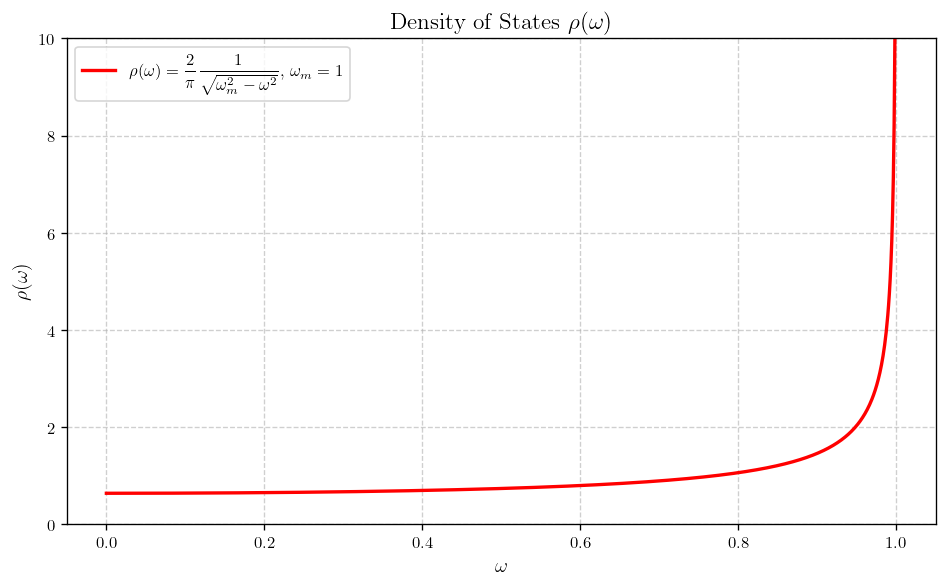
\includegraphics[width=0.7\textwidth]{assets/DOS_1.png}
                \caption{一维单原子链振动的声子态密度}
              \end{figure}
        \item 对于一维双原子链振动,由书P78-79可知色散关系为
              $$\omega_{\pm}^2(q) = \beta\frac{m_2 + m_1}{m_2m_1}\left\{1\pm\left[1 - \frac{4m_2m_1}{(m_2+m_1)^2}\sin^2{\frac{1}{2}qa}\right]^{\frac{1}{2}}\right\}$$
              为得到声子态密度 $\displaystyle\rho(\omega) = \frac{a}{\pi}\left|\frac{\text{d}q}{\text{d}\omega(q)}\right|_{\omega}$,不妨记 $\displaystyle\mu = \frac{m_1m_2}{m_1 + m_2}$,对色散关系两边求导有
              $$2\omega\text{d}\omega = \frac{\dfrac{\beta^2a}{m_1m_2}\sin{qa}\text{d}q}{\dfrac{\beta}{\mu}-\omega^2}$$
              得到
              $$\frac{\text{d}q}{\text{d}\omega} = \frac{\dfrac{2m_1m_2}{\beta^2a}\omega\left(\dfrac{\beta}{\mu}-\omega^2\right)}{\sin{qa}}$$
              由于 $\rho(\omega)$ 是 $\omega$ 的函数,应反解色散关系将 $q(\omega)$ 代入上式,
              $$\sin{qa} = \frac{m_1m_2\omega}{2\beta^2}\sqrt{\left(\frac{2\beta}{m_1} - \omega^2\right)\left(\frac{2\beta}{m_2} - \omega^2\right)\left(\frac{2\beta}{\mu} - \omega^2\right)}$$
              $$\rho(\omega) = \frac{4}\pi\frac{\left|\dfrac{\beta}{\mu} - \omega^2\right|}{\sqrt{\left(\dfrac{2\beta}{m_1} - \omega^2\right)\left(\dfrac{2\beta}{m_2} - \omega^2\right)\left(\dfrac{2\beta}{\mu} - \omega^2\right)}}$$
              \begin{figure}[htbp]
                \centering
                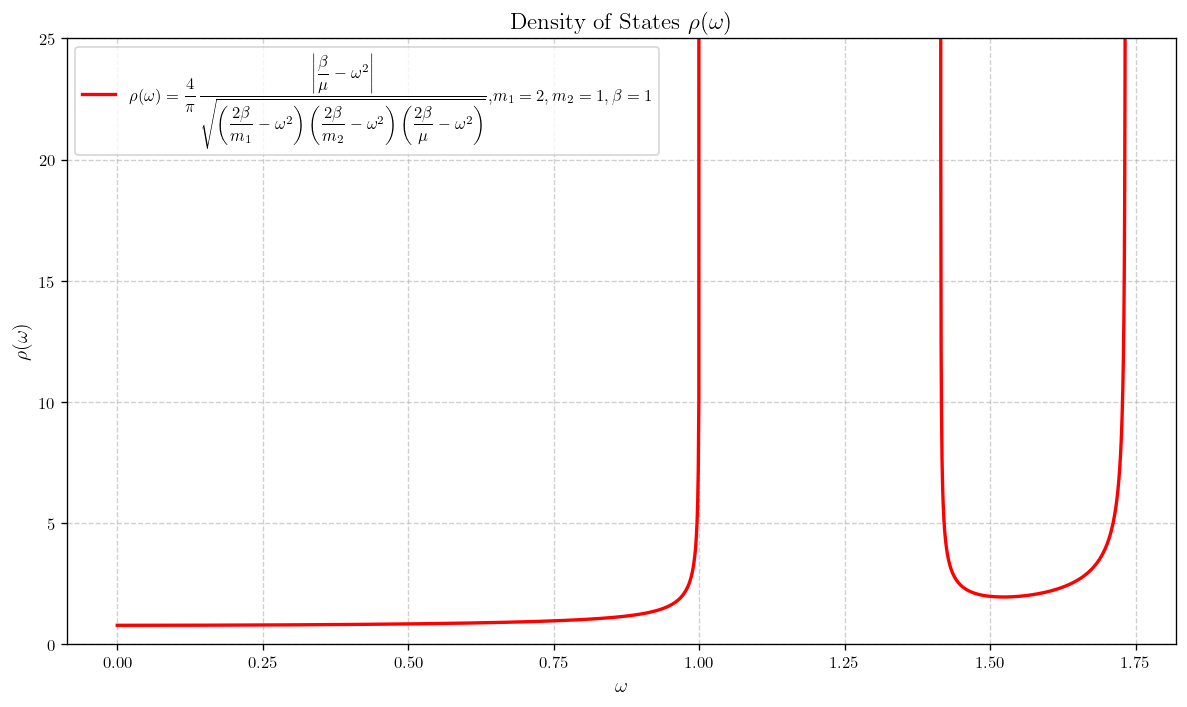
\includegraphics[width=0.7\textwidth]{assets/DOS_2.png}
                \caption{一维双原子链振动的声子态密度}
              \end{figure}
    \end{enumerate}
\end{solution}

\begin{problem}
    设某三维晶体光频支声子的某支色散关系为 $\omega(q) = \omega_0 - Aq^2$,试证明其声子态密度为
    \begin{equation*}
        \rho(\omega) = \left\{
        \begin{aligned}
            &\frac{V}{4\pi^2 A^{\frac{3}{2}}}(\omega_0 - \omega)^{\frac{1}{2}}, &&\omega_{min} < \omega < \omega_0 \\
            &\qquad 0, && \omega > \omega_0 \\
            &\qquad 0, && \omega < \omega_{min}
        \end{aligned}
        \right.
    \end{equation*}
    式中 $\displaystyle\omega_{min} = \omega_0 - A\left(\frac{6\pi^2 N}{V}\right)^{\frac{2}{3}}$,$N$ 为晶体的元胞数。
\end{problem}
\begin{solution}
    根据三维声子态密度
    $$\rho(\omega) = \sum_{q}\delta[\omega - \omega(q)] = \frac{V}{(2\pi)^3}\int\text{d}^3q\delta[\omega - \omega(q)] = \frac{V}{(2\pi)^3}\iint\frac{\text{d}S_\omega}{\left|\nabla\omega(q)\right|}$$
    而 $\omega(q) = \omega_0 - Aq^2$,等频率面为球面,$\displaystyle\iint\text{d}S_\omega = 4\pi q^2$, $\nabla\omega(q) = \dfrac{\text{d}\omega(q)}{\text{d}q} = -2Aq$.
    $$\rho(\omega) = \frac{V}{2\pi^2}q^2\frac{1}{2Aq} = \frac{V}{4\pi^2A}q = \frac{V}{4\pi^2 A^{\frac{3}{2}}}(\omega_0 - \omega)^{\frac{1}{2}}$$
    由声子态密度守恒,
    $$N = \int_{\omega_{min}}^{\omega_0}\rho(\omega)\text{d}\omega = \frac{V}{4\pi^2 A^{\frac{3}{2}}}\left(\frac{2}{3}\right)\left(\omega_0 - \omega_{min}\right)^{\frac{3}{2}}$$
    解得 
    $$\omega_{min} = \omega_0 - A\left(\frac{6\pi^2 N}{V}\right)^{\frac{2}{3}}$$
\end{solution}

\begin{problem}
    设 d 维简单晶格中,声子色散关系 $\omega(\mathbf{q})$ 与 $q^{\mu}$ 成正比,试证明
    \begin{enumerate}[(a)]
        \item 声子态密度 $\rho = B\omega^{\frac{d}{\mu} - 1}$;
        \item 比热容 $C_V = CT^{\frac{d}{\mu}}$。$B$、$C$ 为常量。
    \end{enumerate}
\end{problem}
\begin{solution}
    \begin{enumerate}[(a)]
        \item 设 $\omega(q) = Aq^{\mu}$,由约化声子态密度定义式有
              $$\rho(\omega) = \frac{1}{N} \sum_{q}\delta[\omega - \omega(q)] = \frac{\Omega}{(2\pi)^d}\int\text{d}^qq\delta[\omega - \omega(q)]\varpropto q^{d-1}\left|\frac{\text{d}q}{\text{d}\omega(q)}\right|$$
              故有
              $$\rho(\omega) \varpropto \frac{q^{d-1}}{q^{\mu-1}} \varpropto q^{d-\mu} \varpropto \omega^{\frac{d}{\mu} - 1}$$
              即
              $$\rho = B\omega^{\frac{d}{\mu} - 1}$$
        \item 内能为
              $$U = \int_{0}^{\omega_D}\frac{\hbar\omega}{\text{e}^{\hbar\omega/(K_BT)} - 1}B\omega^{\frac{d}{\mu} - 1}\text{d}\omega = \frac{B(k_BT)^{\frac{d}{\mu}+1}}{\hbar^{\frac{d}{\mu}}}\int_{0}^{\omega_D}\frac{(\dfrac{\hbar\omega}{k_BT})^{\frac{d}{\mu}}\text{d}(\dfrac{\hbar\omega}{k_BT})}{\text{e}^{\hbar\omega/(K_BT)} - 1}$$
              令 $x = \dfrac{\hbar\omega}{k_BT}$,故当 $T\to 0$时,$x\to\infty$,此时积分项近似为常数,故有 
              $$U\varpropto T^{\frac{d}{\mu} + 1} \Longrightarrow C_V = \left(\frac{\partial U}{\partial T}\right)_V = CT^{\frac{d}{\mu}}$$
    \end{enumerate}
\end{solution}

\begin{problem}
    求在一维单原子链中,$\omega > \omega_m$ (截止频率)声子模式的阻尼系数 $\alpha$ 与 $\omega$ 的关系。
\end{problem}
\begin{solution}
    由书P72可得一维单原子链色散关系为
    $$\omega(q) = 2\sqrt{{\frac{\beta}{m}}}\left|\sin{\left(\frac{1}{2}qa\right)}\right|$$
    截止频率 $\displaystyle \omega_m = 2\sqrt{{\frac{\beta}{m}}}$,显然当 $\omega > \omega_m$ 时,$q$应为复数,不妨记 $q = x + iy$,故有
    $$\omega(q) = \pm\omega_m\sin{\left(\frac{1}{2}ax + i\frac{1}{2}ay\right)}$$
    由复数正弦公式
    $$\sin{(x+iy)}= \sin{x}\cdot\cosh{y} + i\cos{x}\cdot\sinh{y}$$
    可以得到
    $$\omega(q) = \pm\omega_m\left(\sin{\frac{1}{2}ax}\cdot\cosh{\frac{1}{2}ay} + i\cos{\frac{1}{2}ax}\cdot\sinh{\frac{1}{2}ay}\right)$$
    由于 $\omega$ 为实数,得到
    $$x = \frac{\pi}{a},\quad \omega = \omega_m\cosh{\frac{1}{2}ay}$$
    代回格波试探解 $\displaystyle u_n = A\text{e}^{i(qna - \omega t)}$ 得到
    $$u_n = A\text{e}^{i\left(\frac{\pi}{a}\pm\frac{2}{a}\cosh^{-1}{\frac{\omega}{\omega_m}}\right)na - i\omega t} = A\text{e}^{in\pi}\text{e}^{2n\cosh^{-1}{\frac{\omega}{\omega_m}}}\text{e}^{-i\omega t}$$
    指数衰减因子\footnote{只有轻杂质才会在能隙内或带边外产生 $\omega > \omega_m$ 的局域模,可在此基础上进行分析。} $\displaystyle\alpha = 2\cosh^{-1}{\frac{\omega}{\omega_m}}$.
\end{solution}
\begin{note}
    复数正弦公式推导:
    \begin{enumerate}
        \item \textbf{定义复数正弦函数}\\  
        基于欧拉公式 $\text{e}^{iz} = \cos z + i \sin z$,复数正弦可定义为:
        $$
        \sin z = \frac{\text{e}^{iz} - \text{e}^{-iz}}{2i}
        $$
        其中 $z = x + iy$($x, y \in \mathbb{R}$)。
    
        \item \textbf{代入复数角度}\\ 
        将 $z = x + iy$ 代入并展开指数项:
        $$
        \begin{aligned}
            \sin(x + iy) &= \frac{\text{e}^{i(x + iy)} - \text{e}^{-i(x + iy)}}{2i} \\
            &= \frac{\text{e}^{-y + ix} - \text{e}^{y - ix}}{2i}
        \end{aligned}
        $$

        \item \textbf{分离实部与虚部}\\
        进一步展开欧拉公式中的三角函数:
        $$
        \begin{aligned}
            \text{e}^{-y} (\cos x + i \sin x) &= \text{e}^{-y} \cos x + i \text{e}^{-y} \sin x, \\
            \text{e}^{y} (\cos x - i \sin x) &= \text{e}^{y} \cos x - i \text{e}^{y} \sin x.
        \end{aligned}
        $$
        代入原式后合并同类项:
        $$
        \sin(x + iy) = \frac{(\cos x)(\text{e}^{-y} - \text{e}^{y}) + i (\sin x)(e^{-y} + \text{e}^{y})}{2i}
        $$
    
        \item \textbf{引入双曲函数}\\
        利用双曲函数的定义 $\displaystyle\cosh y = \frac{\text{e}^{y} + \text{e}^{-y}}{2}$ 和 $\displaystyle\sinh y = \frac{\text{e}^{y} - \text{e}^{-y}}{2}$,化简得到:
        $$
        \begin{aligned}
            \sin(x + iy) &= \frac{-2\cos x \sinh y + i (2 \sin x \cosh y)}{2i} \\
            &= \sin x \cosh y + i \cos x \sinh y
        \end{aligned}
        $$
        最终公式为:
        \begin{equation*}
            \boxed{ \sin(x + iy) = \sin x \cosh y + i \cos x \sinh y }
        \end{equation*}
    \end{enumerate}
\end{note}

\begin{problem}
    格林艾森常数。
    \begin{enumerate}[(a)]
        \item 证明频率为 $\omega$ 的声子模式的自由能为 $k_BT\ln{\left[2\sinh{\left(\dfrac{\hbar\omega}{2k_BT}\right)}\right]}$;
        \item 如果 $\Delta$ 是体积的相对变化量,则晶体的自由能密度可以写为
              $$\displaystyle F(\Delta,T) = \frac{1}{2}B\Delta^2 + k_BT\sum_{q}\ln{\left\{2\sinh{\left[\frac{\hbar\omega(\mathbf{q})}{2k_BT}\right]}\right\}}$$
              其中 $B$ 为体积弹性模量。假定 $\omega(\mathbf{q})$ 与体积关系为 $\dfrac{\text{d}\omega(\mathbf{q})}{\omega(\mathbf{q})} = -\gamma\Delta$,$\gamma$为格林艾森常数,
              且与模 $\mathbf{q}$ 无关。证明当 $\displaystyle B\Delta = \gamma\sum_{q}\frac{1}{2}\hbar\omega(\mathbf{q})\coth{\left[\frac{\hbar\omega(\mathbf{q})}{2k_BT}\right]}$ 时,
              $F$ 对 $\Delta$ 为极小。利用内能密度的定义,证明 $\Delta$ 可近似表达为 $\Delta = \dfrac{\gamma U(T)}{B}$。
        \item 根据德拜模型证明 $\gamma = -\dfrac{\partial\ln{\theta_D}}{\partial\ln{V}}$,其中 $\theta_D = \dfrac{\hbar\omega_D}{k_B}$。
    \end{enumerate}
\end{problem}
\begin{solution}
    \begin{enumerate}[(a)]
        \item 根据书P83-84声子定义可知,晶格振动谐振子能谱为 
              $$E = \hbar\omega\left(n + \dfrac{1}{2}\right)$$
              由书P107-108知系统自由能为
              $$F^V(T,V) = -k_BT\ln{Z^V}$$
              其中 $Z^V$ 为系统的配分函数
              $$Z^V = \sum_n^{\infty}\text{e}^{-\frac{(n+\frac{1}{2})\hbar\omega}{k_BT}} = \frac{\text{e}^{-\frac{\hbar\omega}{2k_BT}}}{1 - \text{e}^{-\frac{\hbar\omega}{k_BT}}}$$
              化简得到
              $$Z^V = \frac{1}{\text{e}^{\frac{\hbar\omega}{2k_BT}} - \text{e}^{-\frac{\hbar\omega}{2k_BT}}} = \left(2\sinh{\frac{\hbar\omega}{k_BT}}\right)^{-1}$$
              故
              $$F^V(T,V) = -k_BT\ln{Z^V} = k_BT\ln{\left[2\sinh{\left(\dfrac{\hbar\omega}{2k_BT}\right)}\right]}$$
        \item 体积为 $V$ 的晶体在有限温度下的自由能由零温时的内能 $U_0(V)$ 和有温度下声子激发贡献的自由能两部分组成,其中零温时的内能可以在平衡体积 $V_0$ 处展开
              $$U_0(V) = U_0(V_0) + U^\prime(V_0)\delta V + \frac{1}{2}U^{\prime\prime}(V_0)\delta V^2$$
              平衡位置处 $U^\prime(V_0) = 0$,体弹性模量 $\displaystyle B = V_0\left(\frac{\partial^2 U}{\partial V^2}\right)$,故内能随体积的变化为
              $$U_0(V) = U_0(V_0) + \frac{1}{2}V_0B\left(\frac{\delta V}{V_0}\right)^2 = V_0\left[\frac{U_0(V_0)}{V_0} + \frac{1}{2}B\Delta^2\right]$$
              这样给定温度和单位体积($V_0 = 1$),亥姆霍兹自由能密度可写为
              $$\displaystyle F(\Delta,T) = \frac{1}{2}B\Delta^2 + k_BT\sum_{q}\ln{\left\{2\sinh{\left[\frac{\hbar\omega(\mathbf{q})}{2k_BT}\right]}\right\}}$$
              要证明当 $\displaystyle B\Delta = \gamma\sum_{q}\frac{1}{2}\hbar\omega(\mathbf{q})\coth{\left[\frac{\hbar\omega(\mathbf{q})}{2k_BT}\right]}$ 时,$F$ 对 $\Delta$ 为极小,有
              $$\frac{\partial F}{\partial \Delta} = B\Delta + k_BT\sum_{\mathbf{q}}\frac{2\cosh{[\hbar\omega(\mathbf{q})/2k_BT]}}{2\sinh{[\hbar\omega(\mathbf{q})/2k_BT]}}\times\frac{\hbar}{2k_BT}\frac{\text{d}\omega(\mathbf{q})}{\text{d}\Delta} = 0$$
              由于 $\text{d}\Delta = \text{d}V$,\ $\dfrac{\text{d}\omega(\mathbf{q})}{\omega(\mathbf{q})} = -\gamma\Delta$,\ 有 $\displaystyle\frac{\text{d}\omega(\mathbf{q})}{\text{d}\Delta} = \frac{\text{d}\omega(\mathbf{q})}{\text{d}V} = -\gamma\omega(\mathbf{q})$,故
              $$B\Delta = \gamma\sum_{q}\frac{1}{2}\hbar\omega(\mathbf{q})\coth{\left[\frac{\hbar\omega(\mathbf{q})}{2k_BT}\right]}$$
              经检验,$\displaystyle \frac{\partial^2 F}{\partial \Delta^2} > 0$,此时确实为自由能极小值。 \\[12pt]
              根据自由能可计算熵
              $$S = -\left(\frac{\partial F}{\partial T}\right)_V = -k_B\sum_{\mathbf{q}}\ln{\left[\left(2\sinh{\frac{\hbar\omega(\mathbf{q})}{2k_BT}}\right)\right]} + \frac{1}{T}\sum_{\mathbf{q}}\frac{1}{2}\hbar\omega(\mathbf{q})\coth{\left(\frac{\hbar\omega(\mathbf{q})}{2k_BT}\right)}$$
              内能密度函数
              $$U(T,\Delta) = F + TS = \frac{1}{2}\Delta^2 + \sum_{\mathbf{q}}\frac{1}{2}\hbar\omega(\mathbf{q})\coth{\left(\frac{\hbar\omega(\mathbf{q})}{2k_BT}\right)}$$
              利用 $\displaystyle B\Delta = \gamma\sum_{q}\frac{1}{2}\hbar\omega(\mathbf{q})\coth{\left[\frac{\hbar\omega(\mathbf{q})}{2k_BT}\right]}$ 得到
              $$U(T,\Delta) = \frac{1}{2}B\Delta^2 + \frac{B\Delta}{\gamma} \approx \frac{B\Delta}{\gamma}$$
              故  $\Delta$ 可近似表达为 $\Delta = \dfrac{\gamma U(T)}{B}$.
        \item 推广的格林艾森常数表达式为 
              $$\gamma = \frac{\displaystyle\sum_{\mathbf{q}s}\gamma_{\mathbf{q}s}C_V^{\mathbf{q}s}}{\displaystyle\sum_{\mathbf{q}s}C_V^{\mathbf{q}s}}$$
              其中 $\displaystyle\gamma_{\mathbf{q}s} = \frac{\partial\ln{\omega_s(\mathbf{q})}}{\partial\ln{V}}$ 是($\mathbf{q}s$)模式的格林艾森常数,$\displaystyle C_V^{\mathbf{q}s}(T)$ 是($\mathbf{q}s$)模式的比热容。 \\[12pt]
              德拜模型是单参量的晶格振动模型,$\omega_D$ 是计及非谐效应的唯一参量。德拜模型隐含假定 $\omega_{\mathbf{q}} = \omega_Df_S(\mathbf{q})$,$f_s(\mathbf{q})$ 是与晶体结构有关的函数,非谐效应只包含在 $\omega_D$中,所以有
              $$\gamma = \frac{\displaystyle\sum_{\mathbf{q}s}\gamma_{\mathbf{q}s}C_V^{\mathbf{q}s}}{\displaystyle\sum_{\mathbf{q}s}C_V^{\mathbf{q}s}} = \frac{\displaystyle\sum_{\mathbf{q}s}\gamma_{D}C_V^{\mathbf{q}s}}{\displaystyle\sum_{\mathbf{q}s}C_V^{\mathbf{q}s}} = \gamma_D$$
              其中 $\displaystyle\gamma_D = -\frac{\partial\ln{\omega_D}}{\ln{V}} = - \frac{\partial \ln{\theta_D}}{\partial\ln{V}}$,其中 $\theta_D = \dfrac{\hbar\omega_D}{k_B}$。
    \end{enumerate}
\end{solution}

\newpage
\section{第四章习题}

\begin{problem}
    求证由 $\delta$ 函数构成的一维周期势场 $\displaystyle V(x) = V_0\sum_{l = -\infty}^{+\infty}\delta(x - la)$ 中,
    单电子能谱由下列克勒尼希-彭尼(Kronig-Penny)关系决定:$\displaystyle\cos{ka} = \dfrac{maV_0\sin{\alpha a}}{\alpha a} + \cos{(\alpha a)}, \alpha^2 = 2mE/\hbar^2$。
    由此结果说明每一能带色散关系均满足 $E(k+K_h) = E(k)$,当 $V_0$ 为负数,该模型是单电子在一维原子链中运动的一种很好的描述。
\end{problem}
\begin{solution}
    
\end{solution}

\begin{problem}
    电子在周期场中的势能
    $$
    V(x) = \left\{
    \begin{aligned}
        &\frac{1}{2}m\omega^2\left[b^2 - (x - na)^2\right], &na - b \leq x \leq na + b \\
        &0, &(n - 1)a + b \leq x \leq na - b
    \end{aligned}
    \right.
    $$
    且 $a = 4b$,$\omega$ 是常量。试画出该势能曲线,并求该势能的平均值。
\end{problem}
\begin{solution}
    
\end{solution}

\begin{problem}
    用近自由电子近似处理上题,求此晶体第一及第二能隙宽度。
\end{problem}
\begin{solution}
    
\end{solution}

\begin{problem}
    设两维正方晶格的周期势为
    $$V(\mathbf{r}) = V(x,y) = - 4U\cos{\frac{2\pi x}{a}}\cos{\frac{2\pi y}{a}}$$
    $a$ 为晶格常量,求:
    \begin{enumerate}[(a)]
        \item $V(\mathbf{r})$ 按倒格矢展开的傅立叶系数 $V(\mathbf{K}_h)$;
        \item 对近自由电子近似而言,在哪些布里渊区界线上有布拉格反射,并写出相应的能隙。
    \end{enumerate}
\end{problem}
\begin{solution}
    
\end{solution}

\begin{problem}
    已知近自由电子近似在布里渊区边界附近能量为
    $$E_{\pm}(\mathbf{k}) = \frac{1}{2}\left\{\left[E^0(\mathbf{k}) + E^0(\mathbf{k} + \mathbf{K}_h)\right] \pm \sqrt{\left[E^0(\mathbf{k}) - E^0(\mathbf{k} + \mathbf{K}_h)\right]^2 + 4\left|V(\mathbf{K}_h)\right|^2}\right\}$$
    证明在布里渊区界面上,垂直于布里渊区界面的电子速度分量为0。
\end{problem}
\begin{solution}
    
\end{solution}

\begin{problem}
    设二维长方晶格的周期势 $\displaystyle V(\mathbf{r}) = V_0 + A\cos{\frac{4\pi x}{a} + B\cos{\frac{2\pi y}{a}}}$,
    试用近自由电子近似求电子状态为 $\displaystyle\mathbf{k} = \left(\frac{2\pi}{a}, k_y\right)$ 的能量及其相应的波函数。
\end{problem}
\begin{solution}
    
\end{solution}

\begin{problem}
    用紧束缚近似方法求出面心立方晶体 s态电子能带
    $$E(\mathbf{k}) = E_s - J_0 - 4J_1\left(\cos{\frac{k_x a}{2}}\cos{\frac{k_y a}{2}} + \cos{\frac{k_y a}{2}}\cos{\frac{k_z a}{2}} + \cos{\frac{k_z a}{2}}\cos{\frac{k_x a}{2}}\right)$$
    并求能带底部的有效质量。
\end{problem}
\begin{solution}
    
\end{solution}

\begin{problem}
    某晶体中电子的等能面是椭球面 $\displaystyle E(\mathbf{k}) = \frac{\hbar^2}{2}\left(\frac{k_x^2}{m_1} + \frac{k_y^2}{m_2} + \frac{k_z^2}{m_3}\right)$,求该能谱的电子态密度。
\end{problem}
\begin{solution}
    
\end{solution}

\newpage
\section{第五章习题}

\begin{problem}
    二维自由电子气系统,每单位面积中的电子数为 $n$,试求出系统的
    \begin{enumerate}[(a)]
        \item 电子能态密度 $N(E)$;
        \item 有限温度下的化学势 $\displaystyle\mu(T) = k_BT\ln{\left[\text{exp}\left(\frac{nh^2}{4\pi mk_BT}\right) - 1\right]}$.
    \end{enumerate}
\end{problem}
\begin{solution}
    
\end{solution}

\begin{problem}
    设阻尼项为 $-m^*\bm{\upsilon}\tau$,试证明当 $\mathbf{E} = (E_x, E_y,E_z), \mathbf{B} = (0, 0, B)$ 时直流电导率公式为
    \begin{equation*}
        \begin{pmatrix}
            J_x \\
            J_y \\
            J_z
        \end{pmatrix}
        =
        \frac{\sigma}{1 + (\omega_c\tau)^2}
        \begin{pmatrix}
            1 & -\omega_c\tau & 0 \\
            \omega_c\tau & 1 & 0 \\
            0 & 0 & 1 + (\omega_c\tau)^2
        \end{pmatrix}
        \begin{pmatrix}
            E_x \\
            E_y \\
            E_z
        \end{pmatrix}
    \end{equation*}
    其中, $\sigma = ne^2\tau / m^*$, $\omega_c = eB / m^*$.
\end{problem}
\begin{solution}
    
\end{solution}

\begin{problem}
    电子漂移速度 $\bm{\upsilon}$ 满足方程 $\displaystyle m^*\left(\frac{\text{d}\bm{\upsilon}}{\text{d}t} + \frac{\bm{\upsilon}}{\tau}\right) = -e\mathbf{E}$。
    试证明频率为 $\omega$ 的电导率为 $\displaystyle\bm{\sigma}(\omega) = \sigma(0)\frac{1 + i\omega\tau}{1 + (\omega\tau)^2}$,其中 $\sigma(0) = ne^2\tau / m^*$.
\end{problem}
\begin{solution}
    
\end{solution}

\begin{problem}
    在低温下实验测出某绝缘体晶体的比热容与温度的关系 $C_V / T^{3 / 2} - T^{3 / 2}$为一直线,斜率为 $B$,截距为 $A$,如图所示。
    \begin{enumerate}[(a)]
        \item 写出低温下 $C_V$ 与 $T$ 关系;
        \item 若已知直线的斜率部分来源于声子对比热容的贡献,求 $B$ 与德拜温度 $\theta_D$ 的关系;
        \item 设截距部分来源于某波色子对比热容的贡献,试估计该准粒子的色散关系中 $\omega(\bm{q})\approx q^\mu$ 的 $\mu$.
    \end{enumerate}
\end{problem}

\end{document}
